\chapter{Introduction}

Nanophotonic devices are key building blocks in emerging technologies such as on-chip lasers, high-speed modulators, and quantum photonic platforms. 
These systems must operate reliably under real-world conditions: lasers must manage thermal and electrical effects, modulators must respond efficiently 
to electrical or thermal signals, and quantum devices need to carefully mitigate (or utilize) mechanical and electromagnetic phenomena. In all these cases, device 
performance arises from the interaction of multiple physical domains, including electromagnetism, heat transfer, mechanics, and carrier dynamics.

Despite this inherently multiphysics nature, most current design approaches treat these effects in isolation or overlook them entirely. Designs are typically optimized 
for idealized optical performance, while non-optical effects are considered only a posteriori,
often resulting in suboptimal or unstable devices. This gap between idealized design models and real-world device behavior limits the scalability and robustness of current nanophotonic technologies.

One reason for this limitation is that conventional design methods rely on well-established, single-physics models (e.g. photonic crystals and waveguides), while the full multiphysics problem remains computationally challenging.
However, when thermal, mechanical, or electrical effects strongly influence the optical response, neglecting them in the design phase can compromise overall device performance.

This Ph.D. project aims to address these challenges by developing and applying multiphysics topology optimization methods for nanophotonic device design. These methods enable the simultaneous treatment of coupled physical effects, 
allowing for the automated discovery of device geometries that are not only optically efficient, but also account and utilize thermal, mechanical, and electrical effects. Beyond improving device reliability, this approach can reveal 
novel design principles and physical phenomena that emerge only when multiple physics are considered simultaneously.

\section{Multiphysics effects in nanophotonics}

Multiphysics effects play a crucial role not only in advanced nanophotonic technologies but are also abundant in nature, where the interplay of optics with mechanics, thermodynamics, and chemistry creates dynamic and functional nano-optical systems.

\begin{figure}[b!]
    \centering
    \makebox[\textwidth][c]{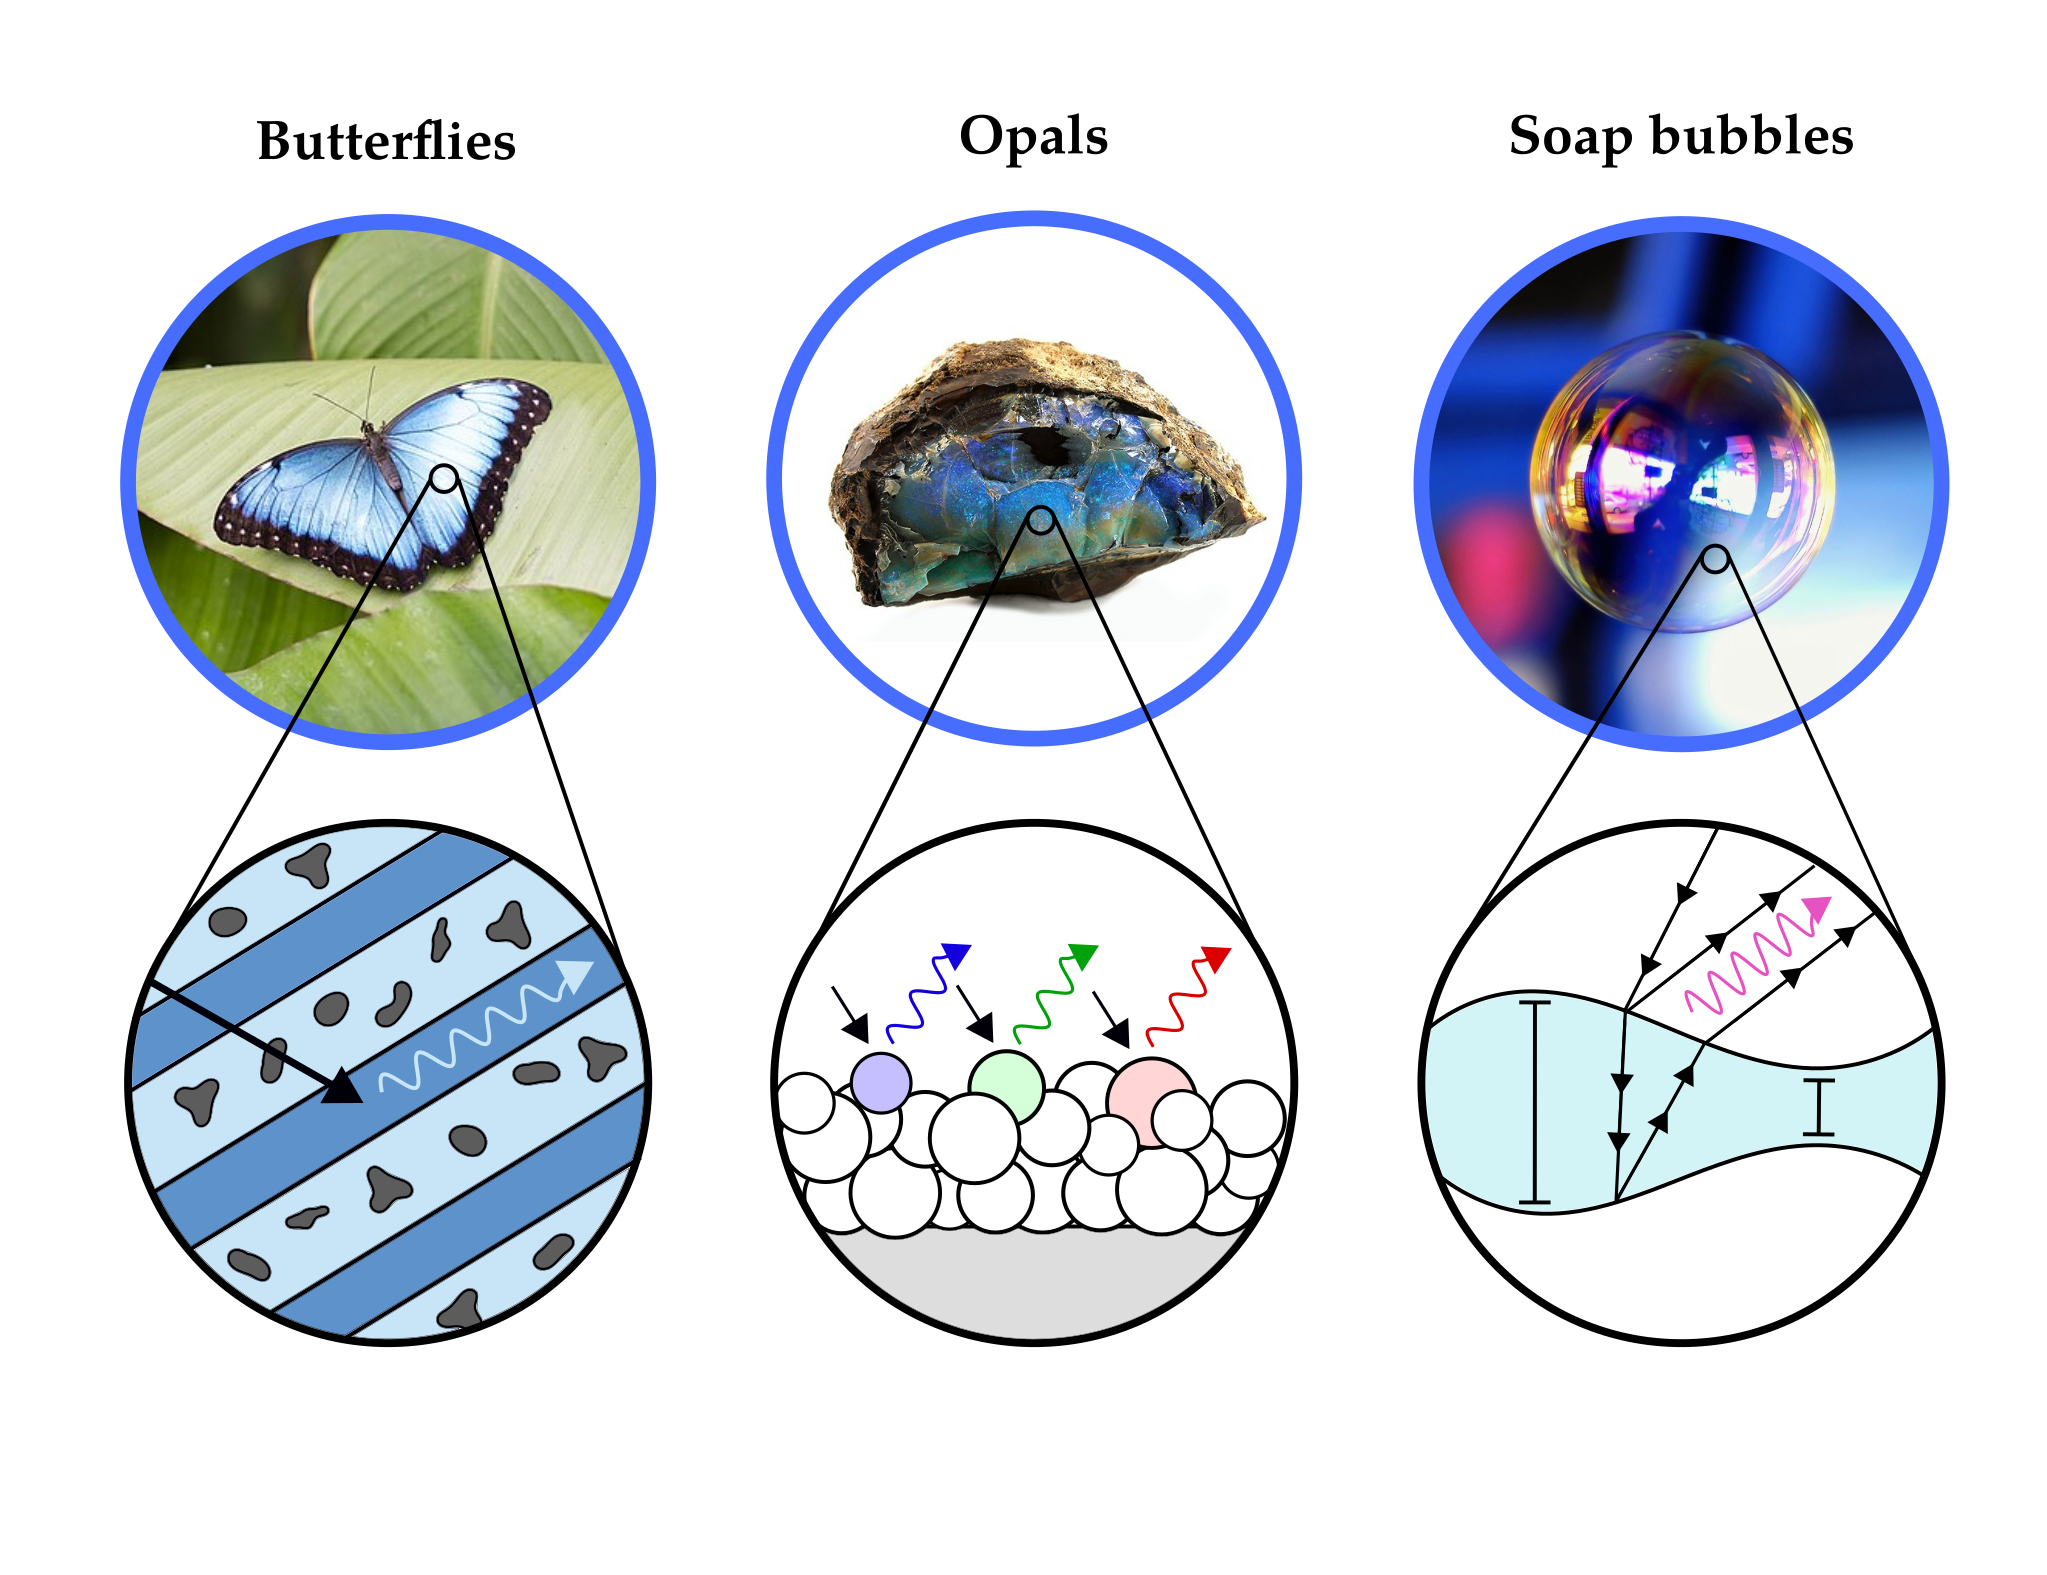
\includegraphics{figures/motivation_natural.png}}%%
    \caption{Common macroscopic examples of nano-optical systems that exhibit multiphysics effects. On the left, the vivid blue color of the \textit{Morpho peleides} butterfly (by Mira Meijer, Burgers' Zoo, \href{https://creativecommons.org/licenses/by-sa/4.0/}{CC BY-SA 4.0}) caused by its nanostructured wings; on the right, the iridescent patterns in soap bubbles (by Jeff Kubina, \href{https://creativecommons.org/licenses/by-sa/2.0/}{CC BY-SA 2.0}) caused by variations in film thickness. Photograph source: \href{https://commons.wikimedia.org/wiki/Main_Page}{Wikimedia commons}.}
    \label{fig:motivation_natural}
\end{figure}

As shown in \figref{fig:motivation_natural} nature provides colourful examples of such multiphysics interactions. For instance, \textit{Morpho peleides} butterfly wings exhibit structural coloration caused by light interacting with nanoscale photonic structures in the wing scales~\cite{butterfly}. This coloration dynamically changes with mechanical deformation of the wings, variations in the angle of light incidence, and environmental factors such as humidity and temperature, which alter the physical properties of the nanostructures. 
Another striking example is the soap bubble, where iridiscent colors arise from thin-film interference effects within the nanoscale thickness of the soap film. The bubble's color shifts as the film thickness changes due to fluid flow, mechanical stresses, evaporation (linked to temperature changes), and chemical composition variations, demonstrating strong coupling between fluid dynamics, thermal and chemical dynamics, and optics.

In engineered nanophotonics, multiphysics coupling is fundamental to a variety of key applications, such as:

\begin{itemize}

\item \textbf{Photonic integrated circuits} (PICs) extensively utilize thermo-optic and electro-optic effects, where electrical signals or temperature changes induce refractive index variations. This enables precise tuning and modulation of optical signals, for optical switching, filtering, and signal processing on compact chips, critical for telecommunications and data processing.

\item \textbf{Nanolasers and light sources} operate through a complex interplay of optical gain, electrical carrier injection, and thermal dissipation. Maintaining stable, efficient lasing requires carefully balancing these coupled phenomena, enabling applications in on-chip light generation and optical communications.

\item \textbf{Sensors} benefit from coupling between electromagnetic fields and mechanical, thermal, or chemical environments. Optomechanical sensors leverage the interaction between light and mechanical motion to achieve exceptional sensitivity to forces, masses, or displacements. Plasmonic and photothermal sensors exploit local field enhancements and environmental effects to detect molecular-scale changes.

\item \textbf{Optical manipulation} refers to the precise control and mechanical actuation of objects using light. This encompasses techniques such as optical trapping of particles, laser cooling to reduce thermal motion, characterization of biomolecules through optical forces, and the use of light pressure for solar sail propulsion and navigation.

\item \textbf{Quantum photonic devices} demand rigorous control of electrical, mechanical, and thermal fluctuations to preserve coherence and enable scalable quantum information processing. Multiphyics effects must be carefully managed to achieve robust quantum state manipulation and measurement.

\end{itemize}

At the intersection of many of these applications, we find \textbf{nano-opto-electro-mechanical systems} (NOEMS)~\cite{NOEMS}, devices that uniquely integrate optical, electrical, and mechanical degrees of freedom at the nanoscale, enabling ultra-compact and highly tunable devices. 
NOEMS exploit the interplay of electrical actuation, mechanical motion, and optical response to realize efficient modulators, switches, sensors, and quantum transducers. 
Together, these examples illustrate that accurately accounting for the coupled multiphysics phenomena is vital for pushing the boundaries of nanophotonic device performance and functionality. CITE ALL THE IMPORTANT STUFF!

% Wikimedia commons:
% 1. https://commons.wikimedia.org/wiki/File:Peleides_blue_morpho_(Morpho_peleides).jpg
% 2. https://commons.wikimedia.org/wiki/File:Opal-53714.jpg
% https://www.reddit.com/r/educationalgifs/comments/56sg9x/a_butterflys_wings_can_change_color_when_soaked/
% Bubble: https://commons.wikimedia.org/wiki/File:Bubble_brokenchopstick.jpg
%Sources:
%The GIF came from this video

%Ding, Y. Structural colors from Morpho peleides butterfly wing scales. J. Appl. Phys. 2009: 106, 074702

%Van Hooijdonk, E., et al. Detailed experimental analysis of the structural fluorescence in the butterfly Morpho sulkowskyi (Nymphalidae) J. Nanophoton. 2011: 5(1), 053525
\section{Topology optimization in nanophotonics}

As illustrated by the examples in the previous sections, ingenously engineered nanostructures and material properties play a crucial role in the
optical response of the system. Inspired by these natural structures an overarching goal of nanophotonic
design is to optimize the geometry and material properties of the system to achieve a desired
optical response.

One powerful approach to address this design challenge is topology optimization~\cite{topopt_book}, a systematich inverse design method used to determine the best way to ditribute 
material within a specified design domain to maximize a specific performance metric, also known as 
objective function or figure of merit (FOM), while satisfying a set of constraints. This method
was pioneered in the field of structural mechanics by Bendsøe and Kikuchi~\cite{bendsoe_kikukchi}, 
and has since been extended to various fields, including fluids~\cite{topopt_fluid}, acoustics~\cite{topopt_acoustic}, 
electromagnetics~\cite{topopt_EM}, (nano)photonics~\cite{topopt_phot}, and multiphysics problems (see \secref{sec:topopt_theory}). In this thesis we focus on the application of density-based~\cite{bendsoe_density, topopt_approaches} 
topology optimization in the field of nanophotonics and nano-optics~\cite{jensen_review}.

Density-based topology optimization describes the distribution of materials within a design space using a 
density field $\rho(\mathbf{r}) \in [0,1]$, where $\rho = 0$ corresponds to one material, typically air or void, and $\rho = 1$ corresponds to a solid material.
 As illustrated 
in \autoref{fig:top_opt} for a nanophotonic system, the objective is to optimize the arrangement of these materials within 
the design domain to achieve a desired performance when illuminated by a light source, such as a laser beam, an LED, or a focused light beam. 
The structure consists of passive regions, where the material remains fixed (e.g. void), and design regions, where the material distribution 
is adjusted through the optimization process. This process iteratively updates the density field until the targeted optical response, 
such as maximizing transmission, reflection, or absorption, is achieved.

\begin{figure}[tb]
    \centering
    \makebox[\textwidth][c]{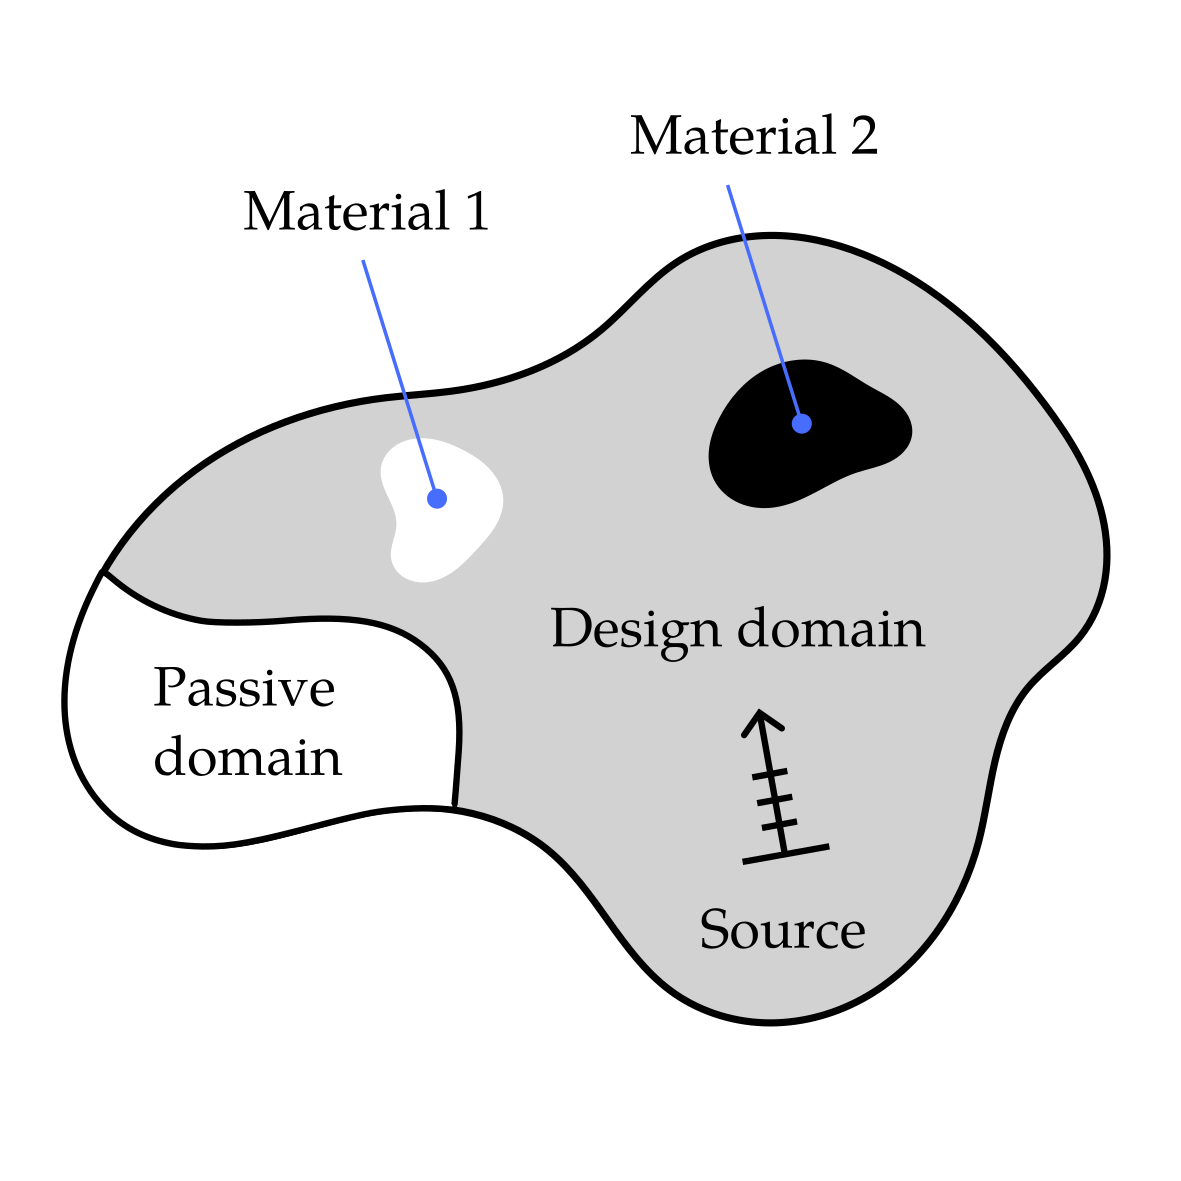
\includegraphics{figures/top_opt.png}}%%
    \caption{Topology optimization of a nanophotonic system, excited by a source. The simulation domain is composed by a passive domain where the material is fixed, and a design domain (grey), where the material distribution is optimized for two different materials.}
        \label{fig:top_opt}
\end{figure}

For further details on inverse design by topology optimization method in photonics and nano-optics, we refer the reader To
the review papers by Jensen and Sigmund~\cite{jensen_review} and the more recent one by Molesky et al.~\cite{Molesky_2018}. 
For a practical introduction to the
the practical implementation of the method we refer to the reader to the tutorial papers 
by Christiansen and Sigmund~\cite{tutorial_matlab, tutorial_COMSOL}.  

\section{Structure of the Thesis}

This thesis covers multiphysics topology optimization problems in nanphotonics. The following three chapters focus on reviewing the main theory, presenting 
the contributions of this thesis in the context of state-of-the-art research.

\textbf{Chapter 2} presents the theoretical framework used in this thesis. This includes the mathematical formalism
to describe the propagation of light in nanophotonic systems, the basics for the numerical implementation for 
finite element-based simulations tools and the theory behind inverse design by topology optimization in multiphysics systems.

\textbf{Chapter 3} presents a review of multiphysics inverse design problem in the context of nanophotonics with special 
focus on the contributions of this thesis.

\textbf{Chapter 4} concludes the thesis with a summary of the main contributions and findings, and discusses the main challenges
and future work in the field of multiphysics topology optimization in nanophotonics.

This thesis consists of a collection of papers, including unpublished work on
strongly coupled optomechanical systems. The published and unpublished content is included in the attached
papers and manuscripts.